\documentclass[pdftex,12pt,a4paper]{article}

\usepackage{graphicx}  
\usepackage[margin=2.5cm]{geometry}
\usepackage{breakcites}
\usepackage{indentfirst}
\usepackage{pgfgantt}
\usepackage{pdflscape}
\usepackage{float}
\usepackage{epsfig}
\usepackage{epstopdf}
\usepackage[cmex10]{amsmath}
\usepackage{stfloats}
\usepackage{multirow}

\renewcommand{\refname}{REFERENCES}
\linespread{1.3}

\usepackage{mathtools}
%\newcommand{\HRule}{\rule{\linewidth}{0.5mm}}
\thispagestyle{empty}
\begin{document}
\begin{titlepage}
\begin{center}
\textbf{}\\
\textbf{\Large{ISTANBUL TECHNICAL UNIVERSITY}}\\
\vspace{0.5cm}
\textbf{\Large{COMPUTER ENGINEERING DEPARTMENT}}\\
\vspace{2cm}
\textbf{\Large{BLG 222E\\ Computer Organization \\ Project 1}}\\
\vspace{2.8cm}
\begin{table}[ht]
\centering
\Large{
\begin{tabular}{lcl}
\textbf{PROJECT DATE}  & : & 12.04.2023\\
\end{tabular}}
\end{table}
\vspace{1cm}
\textbf{\Large{GROUP MEMBERS:}}\\
\begin{table}[ht]
\centering
\Large{
\begin{tabular}{rcl}
number  & : & name \\
150220762  & : & Muhammed Yusuf Mermer  \\
number  & : & name \\
\end{tabular}}
\end{table}
\vspace{2.8cm}
\textbf{\Large{SPRING 2023}}

\end{center}

\end{titlepage}

\thispagestyle{empty}
\addtocontents{toc}{\contentsline {section}{\numberline {}FRONT COVER}{}}
\addtocontents{toc}{\contentsline {section}{\numberline {}CONTENTS}{}}
\setcounter{tocdepth}{4}
\tableofcontents
\clearpage

\setcounter{page}{1}
\section{INTRODUCTION}


\section{IMPLEMENTATIONS AND EXPLANATIONS }
\subsection{Part 2}
\subsubsection{Part 2.c}
In part 2c, we implemented Adress Register File (ARF) using registers we implemented at 
very begining. As a parameter values, we gave registers 8 bits as 8 bit is necesarry for 
implementing PC, AR, SP and PCPast. Besides, of enable and clock these registers 
already supports funsel and load capabilities, which works as specified in part 2.a. 
Therefore, we can directly send clock, funsel and load informations coming from 
input of this module to these registers without writing them again explicitly.

However, for the rsel, like in the part 2.b we will send individual bits to the enables of
the registers. As in the insturction, if a bit comming to the enable is 1, then operation
decleared by funsel will be done.

All 8-bit of information coming from these registers are connected to 16 multiplexers.

First 8 of them used for getting result of outA and other 8 used for getting result of 
outB. Which of these groups takes inputs with same patterns.

What these multipexers do is that they take significatly same digits of different registers 
as inputs and output the bit of a register that wanted by outasel or outbsel. As specified
in the part 2.c; 00 gives AR's bits,01 SP's bits, 10 PCPrev's bits,11 PC's bits. 
These two 8 bits comming from multipexers concatinated in outa and outb and gaved as
the output of the module.

\textbf{inputs:}    clk(1 bit),
load(8 bits),
outasel(2 bits),
outbsel(2 bits),
funsel(2 bits),
rsel(4 bits)

\textbf{outputs:}    
outa(8 bits),
outb(8 bits)

\textbf{module name:} arf



\subsection{Part 4}
In this part, our purpose is to combine all previously made modules. 
At first we started with adding memory module that provided. We see that when 
we are in the write mode it gives high impedance as output and in the read mode
 we cannot change what is inside of memory.

 Our first thought about this is we will write a test bench, so that IR will not
  take input from memory when memory is in the write mode. Not only IR but also 
  two Multiplexer is also taking input from memory which we want to avoid when 
  memory is in writing mode. We did not implemeted our test bench because we saw
   that test bench is already shared one day later (the day we were thinking to 
   start implemeting).

   After adding module of memory, we defined wires that comes into/ goes out of 
   memory. Adress and outALU is not currently output of any other module. 

   At first we did not thought that nearly every wires have to be senesed as 
   output as test bench required. Therefore, initally we made them as intermadiate 
   wires. Then after we see the output wire names, we changed nearlly all our wires' 
   name and make them output.

	For the connection of IR, we gave 8 least signficant bits to the Multiplexer A.
	At our initial design we output IR's most signficant 8 bits from system but later we change
	 it so that it outputs all 16 bits as outputs.

	After IR, we add modules of Multiplexer A and Multiplexer B. Even though 
	Multiplexer is already implemented for previous parts, we cannot use them 
	directly because they are just 1 bit which in case of use, make our module
	complicated. Hence, we made another module for four to one Multiplexer which 
	takes and gives 8 bit values. Not only four two one multiplexer, but also two
	to one multiplexer which also processing 8 bit values had been made to use on 
	multiplexer C. 

	After connecting relevant wires to multiplexers, we added ARF to the system.
	We add new inputs to the system so that we can modify outputs of the ARF.

	With the addition of this module we see that order of call of modules inside of another 
	module does not important if there is exist intermadiate signals (wires), because
	ARF depends on memory via multiplexer and memory depends on ARF through memory
	 address information.

	 Later we add register file and multipexer C to the system. And we made the connections.

	For the ALU at first we make sepearated flag register but due to input and outputs of ALU 
	is strictly given, we connot write sepearated cin input for ALU which directed us to use a register
	inside of ALU module for flag. Then we made proper input and output connections to the ALU
	module.

	


	\textbf{inputs:}
	ARFOutASel(2 bit), ARFOutBSel(2 bit), IRFunsel(2 bit), ARFFunSel(2 bit),
	RFFunSel(2 bit), ALUFunSel(4 bit), RFRSel(4 bit), ARFRSel(4 bit),
	Clock(1 bit), MemWR(1 bit), MemCS(1 bit), IREnable(1 bit),
	IRLH(1 bit), MuxASel(2 bit), MuxBSel(2 bit), MuxCSel(1 bit),
	RFOutASel(3 bit), RFOutBSel(3 bit), RFTSel(4 bit)


	\textbf{outputs:} 
	AOut (8 bits),
    BOut (8 bits),
    ALUOut (8 bits),
    ALUOutFlag (4 bits),
    ARFAOut (8 bits),
    Address (8 bits),
    MemoryOut (8 bits), 
    MuxAOut (8 bits), 
    MuxBOut (8 bits),
    MuxCOut (8 bits),
    IROut (16 bits)

	\textbf{module name:} ALUSystem







\section{DESIGN PHOTOS}
\subsection{Part 2}
\subsubsection{Part 2.c}
\begin{figure}[H]
	\centering
	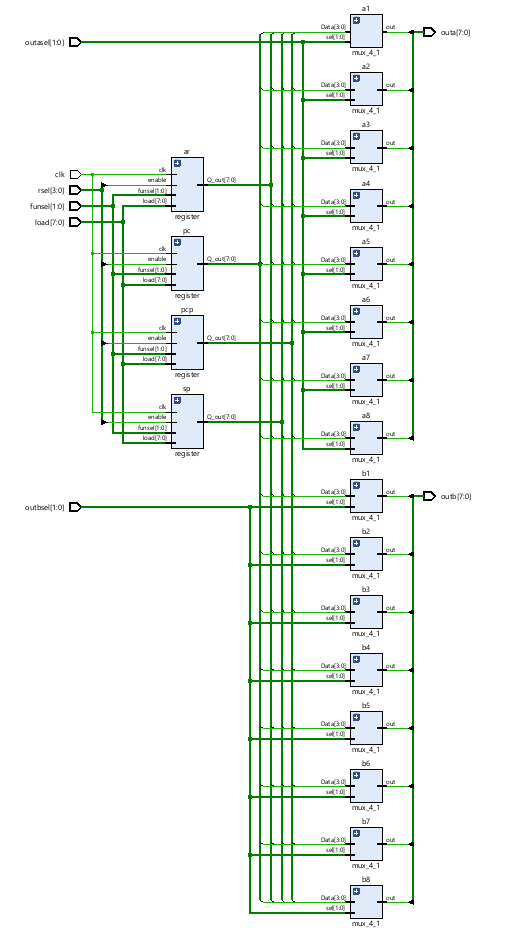
\includegraphics[width=0.5\textwidth]{design/arf.png}	
	\caption{ARF System Design}
	\label{ARF System Design}
\end{figure}

\subsection{Part 4}
    \begin{figure}[H]
    	\centering
    	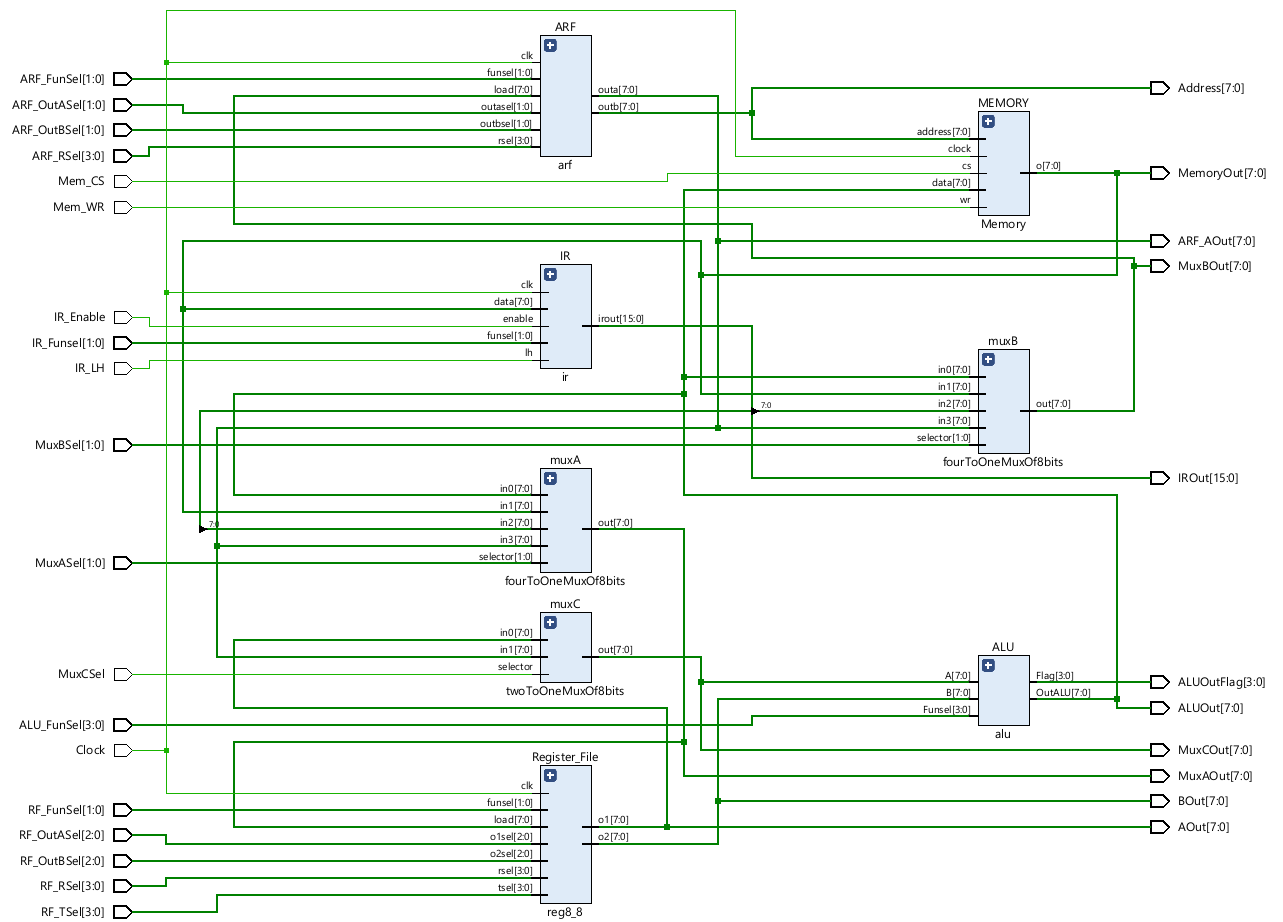
\includegraphics[width=0.9\textwidth]{design/ALU_system.png}	
    	\caption{ALU System Design}
    	\label{ALU System Design}
    \end{figure}








\section{RESULTS}
\subsection{Part 2}
\subsubsection{Part 2.c}
\begin{figure}[H]
	\centering
	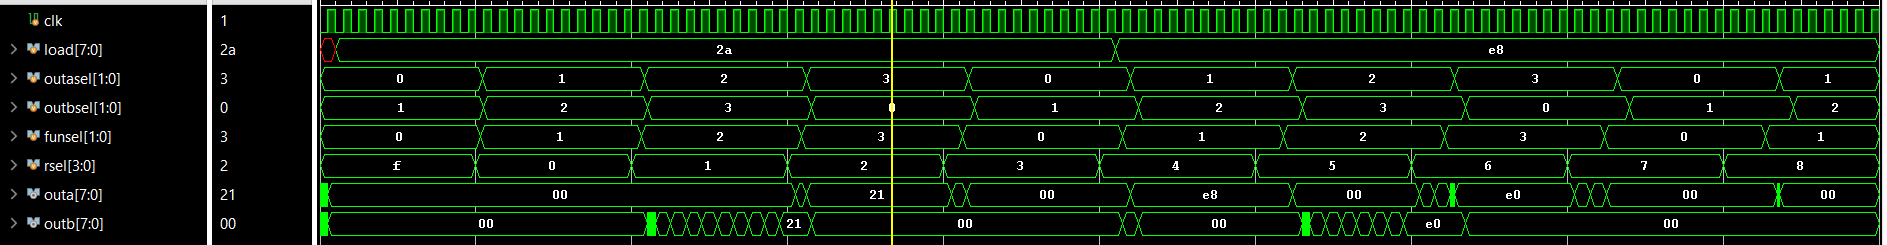
\includegraphics[width=1\textwidth]{results/arf.png}	
	\caption{ARF Simulation}
	\label{ARF Simulation}
\end{figure}


\subsection{Part 4}
result of the part 4 is still contreversial so we will wait for it.


\section{CONCLUSION}

\end{document}

